\documentclass{article}

\usepackage{graphicx}

\setlength{\parskip}{\medskipamount}

\title{Advanced Object Oriented Programming and Design\\
\medskip
\large Homework 3}
\author{Abraham Murciano and Daniel Klein}

\begin{document}

\maketitle

\section{Part A}

The figure below shows the state diagram implementing the requirements specified in the question paper.

\begin{figure}[ht]
	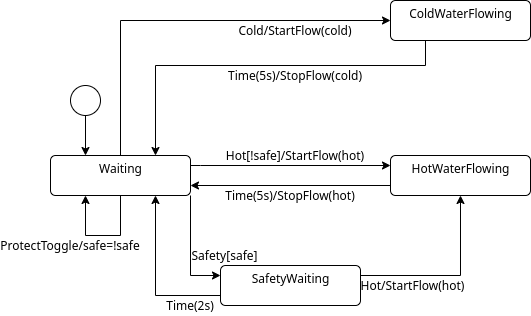
\includegraphics[width=\textwidth]{state-chart.png}
\end{figure}

\section{Part B}

This figure shows a sequence diagram for the case study given in the question paper.

\begin{figure}[ht]
	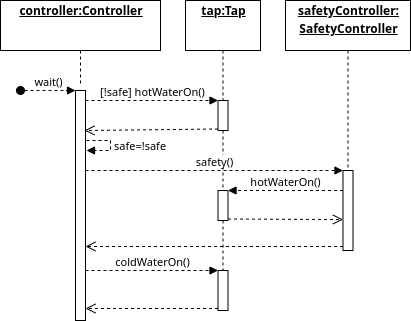
\includegraphics[width=\textwidth]{sequence-diagram.png}
\end{figure}

\section{Part C}

We can add a parameter to the constructor of the water bar and the child protection classes which controls the initial state of the child protection mechanism. The design principle which we considered when applying this change is the Open-Closed Principle, since we want our system to be open to extension by allowing different initial states, but closed to change since if we decide to change the initial state of the child protection, then the water bar class will not have to be recompiled since it uses the same child protection class, just passing it a different value into the constructor.

\end{document}